% 日本語版（ストーリーライン確認用の全訳）。英語版 main.tex と同じ内容・同じ数値。図は英語版と共通。
% 作り方: cd paper && latexmk -xelatex main_ja.tex
\documentclass[conference]{IEEEtran}
\IEEEoverridecommandlockouts
\usepackage{xeCJK}
\setmainfont{TeX Gyre Termes}
\setCJKmainfont{Noto Serif CJK JP}
\setCJKsansfont{Noto Sans CJK JP}
\setCJKmonofont{Noto Sans CJK JP}
\usepackage{cite}
\usepackage{amsmath,amssymb,amsfonts}
\usepackage{graphicx}
\usepackage{booktabs}
\usepackage{xcolor}
\usepackage[hidelinks]{hyperref}
\usepackage{url}
\linespread{1.08}

\newcommand{\Ours}{Ours}
\newcommand{\Unc}{MaxUnc}
\newcommand{\Rand}{Random}
\newcommand{\Geom}{Ours-Threshold}
\newcommand{\Fix}{Ours-FixedShape}

\IfFileExists{author.tex}{\input{author}}{\newcommand{\AuthorName}{AUTHOR NAME}\newcommand{\AuthorEmail}{EMAIL}}

\begin{document}

\title{棚の奥などで一部しか見えない部品を\\掴むためにどこを触るか：\\触った後に掴める確率が最も上がる所を触る}

\author{\IEEEauthorblockN{\AuthorName}
\IEEEauthorblockA{Independent Researcher\\
Japan\\
\AuthorEmail}}

\maketitle

\begin{abstract}
棚に置かれた小部品は、手前しか見えないことが多い。上の段の天板が頭部カメラから奥を隠し、その隠れた部分の形が、どこを挟めば持ち上がるかを決める。本研究は、形ではなく掴むことのために選んだ1回の軽い触りでこれを解決する。形の候補（粒子）を領域分割と深度から作り、物理の値をばらつかせた8,000回のシミュレーションの把持で学習した小さなニューラルネットが、各候補・各挟む点の把持成功確率を予測する。ロボットは、触った後の最良の把持成功確率の期待値が最大になる点を触る。つまり、当たりでも外れでも、次にどこを掴めばよいかがはっきりする所を触る。MuJoCo 上の人型ロボット Unitree G1 と3指ハンドで、240の配置を対応のある比較で評価した。1回触った時点の把持成功率は、本手法 95.4\%、形の不確かさが最大の所を触る規則 88.8\%、ランダム 88.8\% であった（差 +6.7 ポイント、95\% 信頼区間 [+2.1, +11.3]、McNemar 検定 $p=0.005$）。部品が 10\,mm しか見えないとき、差は +15.0 ポイントに広がった。ニューラルネットの代わりに、予備実験の試し掴みから決めた境目3つの見積もりを使っても、同じ先読みで 93.8\% となり、本手法との差は +1.7 ポイント（95\% 信頼区間 [$-$1.3, +4.6]、$p=0.424$）にとどまった。この部品の族はニューラルネットを要するほど難しくなく、成功率を上げたのは触る場所である。同じ先読みのまま、部品の形を中央の寸法に決め打ちして位置と向きだけを推定すると（物体の形を既知とする場合にあたる）、76.7\%（本手法より 18.8 ポイント低い）となった。触らずに掴むと成功率は 72.5\% で、失敗した把持の多くで部品が 10\,mm 以上動いた。予測した成功確率が閾値を超えたら触るのをやめる規則は、毎回1回触る場合と差がなかった。結果はすべてシミュレーションによる。コード、学習済みモデル、生の結果を公開している。
\end{abstract}

\section{はじめに}

工場や倉庫で人型ロボットに部品を取らせるとき、部品はしばしば棚の奥に置かれている。上の段の天板が頭部カメラの視界を遮るので、部品の手前しか見えない。隠れた奥の形が、どこを挟めば持ち上がるかを決めている場合、見えた部分だけから計画した把持は失敗する。さらに棚の下では、失敗の損も大きい。掴み損ねた手を引き出すときに、部品を引きずったり弾いたりする。本研究のシミュレーションでは、失敗した把持の 91\% で部品が 10\,mm 以上動いた（\ref{sec:cost} 節）。失敗から学ぶより、掴む前に軽く触って形を確かめる方が安全である。

一部が見えた形を触覚で補ってから掴む研究は多い~\cite{rustler2022actvh,rustler2023efficient,defarias2021simultaneous,rustler2026shapegrasp}。その多くは、形の不確かさが最大の所を触る~\cite{rustler2022actvh,dragiev2013uncertainty,kissoum2023tactile}。この基準は形を復元するには理にかなっているが、掴むためには必ずしも最善ではない。最も不確かな所が、掴めるかどうかと関係のない所（たとえば部品の奥の端）であることがあるからである。

本研究は、\emph{触った後の最良の把持成功確率の期待値}が最大になる点を触る。平たく言えば、当たりでも外れでも、次にどこを掴めばよいかがはっきりする所を触る。各形の候補・各挟む点の成功確率は、摩擦・質量・指のゲインをばらつかせた物理シミュレーションの試行から学習した小さなニューラルネットで出す。それを Lundell ら~\cite{lundell2019robust} と同じく候補で平均するが、本研究はそれを掴む点だけでなく触る点の選択にも使う。DA-GRD~\cite{wang2026dagrd} も、物体の空間ではなく把持の空間で探るが、対象は認識から実行までの間に位置がずれた既知の物体であり、把持は幾何の許容幅で判定する。本研究が扱うのは、棚の下で隠れた\emph{形}である。触る点の選び方は、候補ごとの成功確率の見積もりであれば何でも使える。本研究では、ニューラルネットと、予備実験の試し掴みから決めた境目3つの見積もりを比べた。この部品の族では、掴めるかどうかが挟む点が本体の縁からどれだけ内側にあるかでほぼ決まるので、簡単な見積もりでもほぼ同じ成功率になった。形の不確かさを基準に触る規則に対する利点は、掴むための基準そのものから生じている。

本研究の貢献は次の3つである。
\begin{enumerate}
\item 一部が隠れた部品を掴むための触る点の選び方。部分的な視覚と軽い接触から形の候補を作り、触った後の最良の把持成功確率の期待値で触る点を評価する。
\item 棚の下の人型ロボットでの、240配置の対応のある評価。天板は部品を隠すと同時に、手の入り方も制約する。2つの要素はどちらも必要である。触る基準だけを形の不確かさに変えると 6.7 ポイント、形を中央の寸法に決め打ちして位置だけを推定すると 18.8 ポイント下がる。ニューラルネットの代わりに境目3つの見積もりを使っても、形の不確かさの基準を +5.0 ポイント（$p=0.050$）上回る。成功率の差は、見積もりの細かさではなく、基準と形の推定から生じている。
\item 簡単な選択で足りる条件の分析。この部品の族では、境目3つの見積もりとニューラルネットの差は +1.7 ポイント（有意差なし）であり、1回触れば足りる。そのため、触る回数を成功確率の閾値で決める規則は、毎回1回触る場合と差がない。
\end{enumerate}

\section{関連研究}

\textbf{視覚と触覚で形を補って掴む。} Act-VH~\cite{rustler2022actvh} は、カメラ1視点の形を暗黙関数のニューラルネットで補完し、補完のばらつきが最大の所を触る。実機の2指グリッパーで、5回触ると把持成功率が 38\% から 80\% に上がった。VISHAC~\cite{rustler2023efficient} はその高速版である。いずれも触る回数は固定で、物体は机に固定されている。de Farias ら~\cite{defarias2021simultaneous} は形をガウス過程の陰関数曲面で表し、把持の試行の接触で形を直す。ShapeGrasp~\cite{rustler2026shapegrasp} は触らずに掴み、失敗した後の指の接触から形を直す。把持は、補完した1つの形に対して物理シミュレーションで評価する。触覚だけを使う方法~\cite{kamtikar2026tactful,pai2023tactofind,kissoum2023tactile} は、物体の位置推定・識別・形の復元を行う。本研究は、部分的な視覚で候補を絞り、触る点を掴むための基準で選ぶ。

\textbf{不確かさの下での把持。} Lundell ら~\cite{lundell2019robust} は、ドロップアウトで得た形の候補で把持の質を平均して頑健な把持を選ぶが、触らない。Dex-Net 2.0~\cite{mahler2017dexnet2} は、大量の合成データから把持の成功を学習する。Hsiao ら~\cite{hsiao2011robust} は、物体の位置の信念を持ち、掴みながら触覚で更新する。本研究の成功確率の見積もりは、形の候補ごとに物理の試行から学習し、摩擦・質量・指の制御のばらつきは学習データの中で平均する。

\textbf{目的に向けた能動的な探索。} Dragiev ら~\cite{dragiev2013uncertainty} は、GPIS の分散から「探る把持」と「確実な把持」を作るが、両者の切り替え方は扱っていない。Kissoum~\cite{kissoum2023tactile} は、形の情報量で触覚の探りを選び、復元の精度で評価する。DA-GRD~\cite{wang2026dagrd} は、把持が支持されるまでだけ位置の信念を絞り込み、探りを把持の空間で幾何の許容幅を使って評価する。Learning to Grasp Without Seeing~\cite{murali2018grasp} は、パーティクルフィルタで作業面を触覚で走査する。視覚の側では、能動知覚のベンチマークや方策が、カメラを動かして隠れた視界を取り戻す~\cite{luo2026recovering,liu2026sapave}。本研究は DA-GRD と同じく掴むことを目的とするが、未知なのは隠れた形である。形を中央の寸法に決め打ちした位置だけの版（\Fix）で、形を推定することの価値を測る。

\textbf{隠れと触覚。} Jiang ら~\cite{jiang2026touchmatter} は、散らかりや隠れが増えるほど触覚と力が重要になることを実機で示した。Caddeo ら~\cite{caddeo2026physgen} は、手による隠れの下で、関節の感覚と複数点の接触から形を復元する。DexTacWAM~\cite{yuan2026dextacwam} は、視覚と触覚の世界行動モデルで隠れた物体を掴み、成功したデモだけでは探る動作や立て直しを学べないことを指摘している。これらはいずれも、物体自身・手・周りの物に隠された机の上の物体を扱っており、物体を隠すと同時に手の入り方も制約する棚の天板は扱っていない。

\section{問題設定}

\textbf{形の族。} 部品は、手前の低いフランジ（高さ 4\,mm）と、その奥の掴める本体（幅・高さ $W=20$\,mm）をつないだ1つの剛体である。形の型は既知とし、フランジの長さ $\ell_f\in[10,30]$\,mm と本体の長さ $\ell_b\in[12,20]$\,mm を未知とする。状態は
\begin{equation}
\theta=(x_f, y, \psi, \ell_f, \ell_b)
\end{equation}
で、$(x_f,y)$ は手前の面の中心、$\psi$ は向きである（図~\ref{fig:shapes}）。部品の軸に沿った座標 $a$ で、本体は $a\in[\ell_f,\ell_f+\ell_b]$ を占める。フランジだけを挟んでも部品は持ち上がらない。

\textbf{見え方。} 部品は、机の上 20\,cm にある天板の下に置かれる。フランジの上面が見える長さ $v$ を $v\in\{10,15,20,25\}$\,mm とする。$v=10$\,mm では本体は常に見えず、$v=25$\,mm では配置の 55\% で本体の手前の縁がカメラに見える。

\begin{figure}[t]
\centering
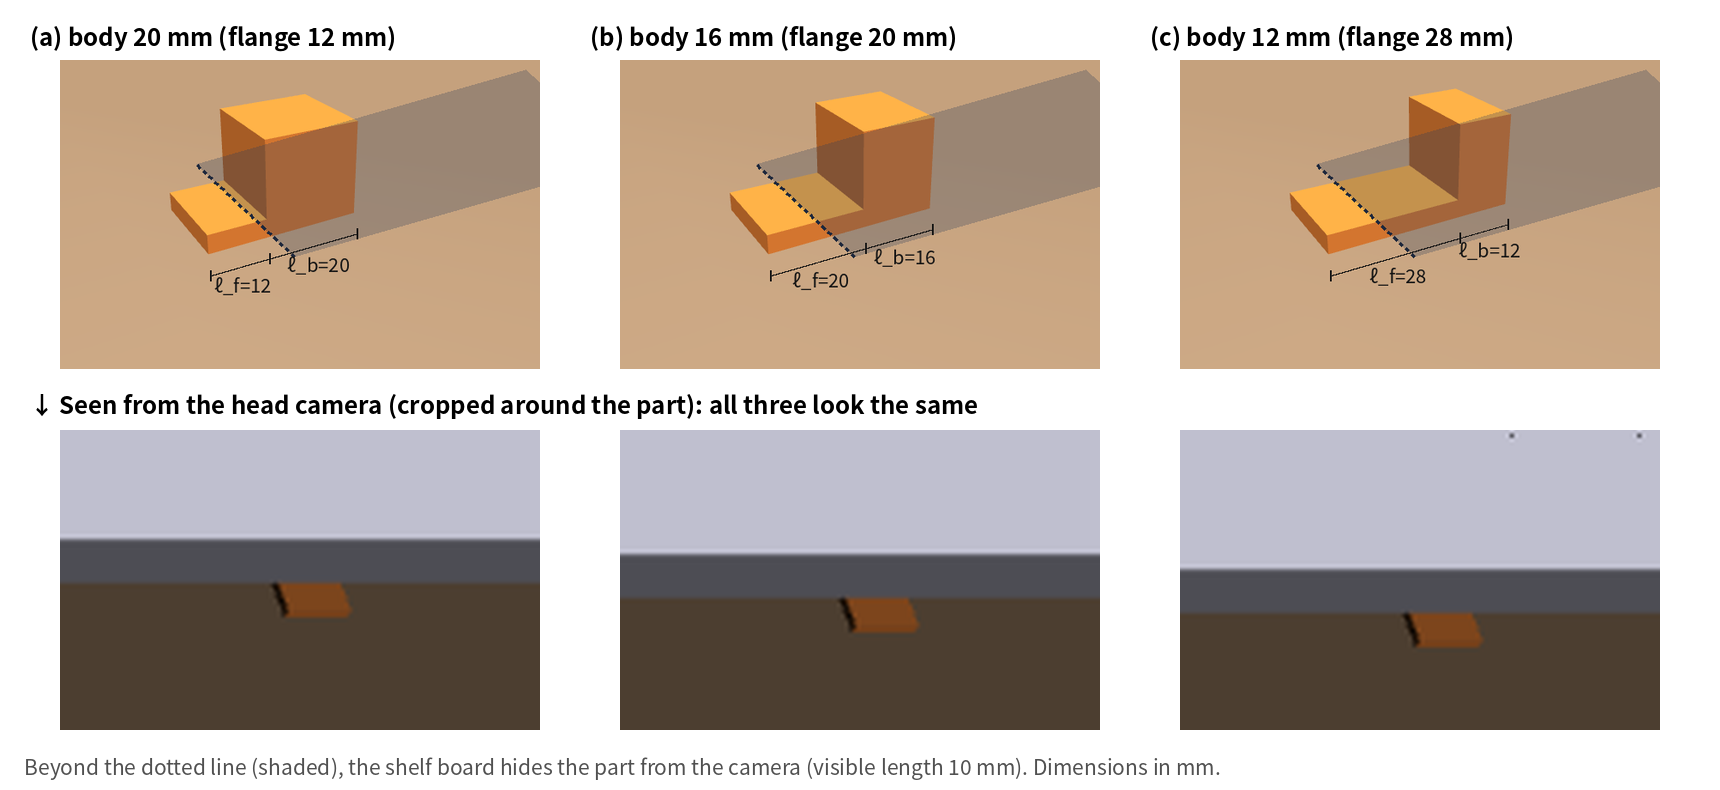
\includegraphics[width=\linewidth]{figures/shapes.png}
\caption{形の族。上：フランジと本体の長さが違う3つの部品（MuJoCo の描画）。点線より奥は天板に隠れる。下：同じ配置を頭部カメラから見た画像。フランジの手前しか見えず3つは区別できないが、挟むべき所は本体がどこから始まるかで変わる。}
\label{fig:shapes}
\end{figure}

\textbf{観測。} ロボットはまず頭部カメラから領域分割と深度を得る。点 $u$ を上から軽く触ると、次の4通りの結果のどれかを得る。
\begin{equation}
o\in\{\textsc{miss},\ \textsc{body-center},\ \textsc{body-other},\ \textsc{flange}\}
\end{equation}
\textsc{miss} は外れ、\textsc{body-center} は指先の中央が本体に当たったこと、\textsc{body-other} は指のそれ以外の所（主に指の腹）が本体に当たったこと、\textsc{flange} はフランジに当たったことを表す。

\textbf{把持と成功。} 把持では、天板の下で手を挟む点 $g$ の真上へ運び、中指と親指で挟み、部品を引き出して持ち上げる。成功 $S=1$ は、2秒保持した後に部品が初期の高さより 4\,cm 以上高いことである。成否は $\theta$、$g$、観測できない物理の値 $\xi$（摩擦、質量、指の制御ゲイン）に依存する。

\textbf{目的。} $k$ 回触った後の把持成功率を最大にする触る点を選ぶ。主な評価は $k=1$ で行う。

\section{手法}

$\theta$ の信念を粒子 $\{\theta_i\}_{i=1}^{N}$（$N=200$）で表し、カメラで初期化して、触るたびに更新する。触る点と掴む点は、粒子で平均した成功確率から選ぶ（図~\ref{fig:pipeline}）。

\begin{figure*}[t]
\centering
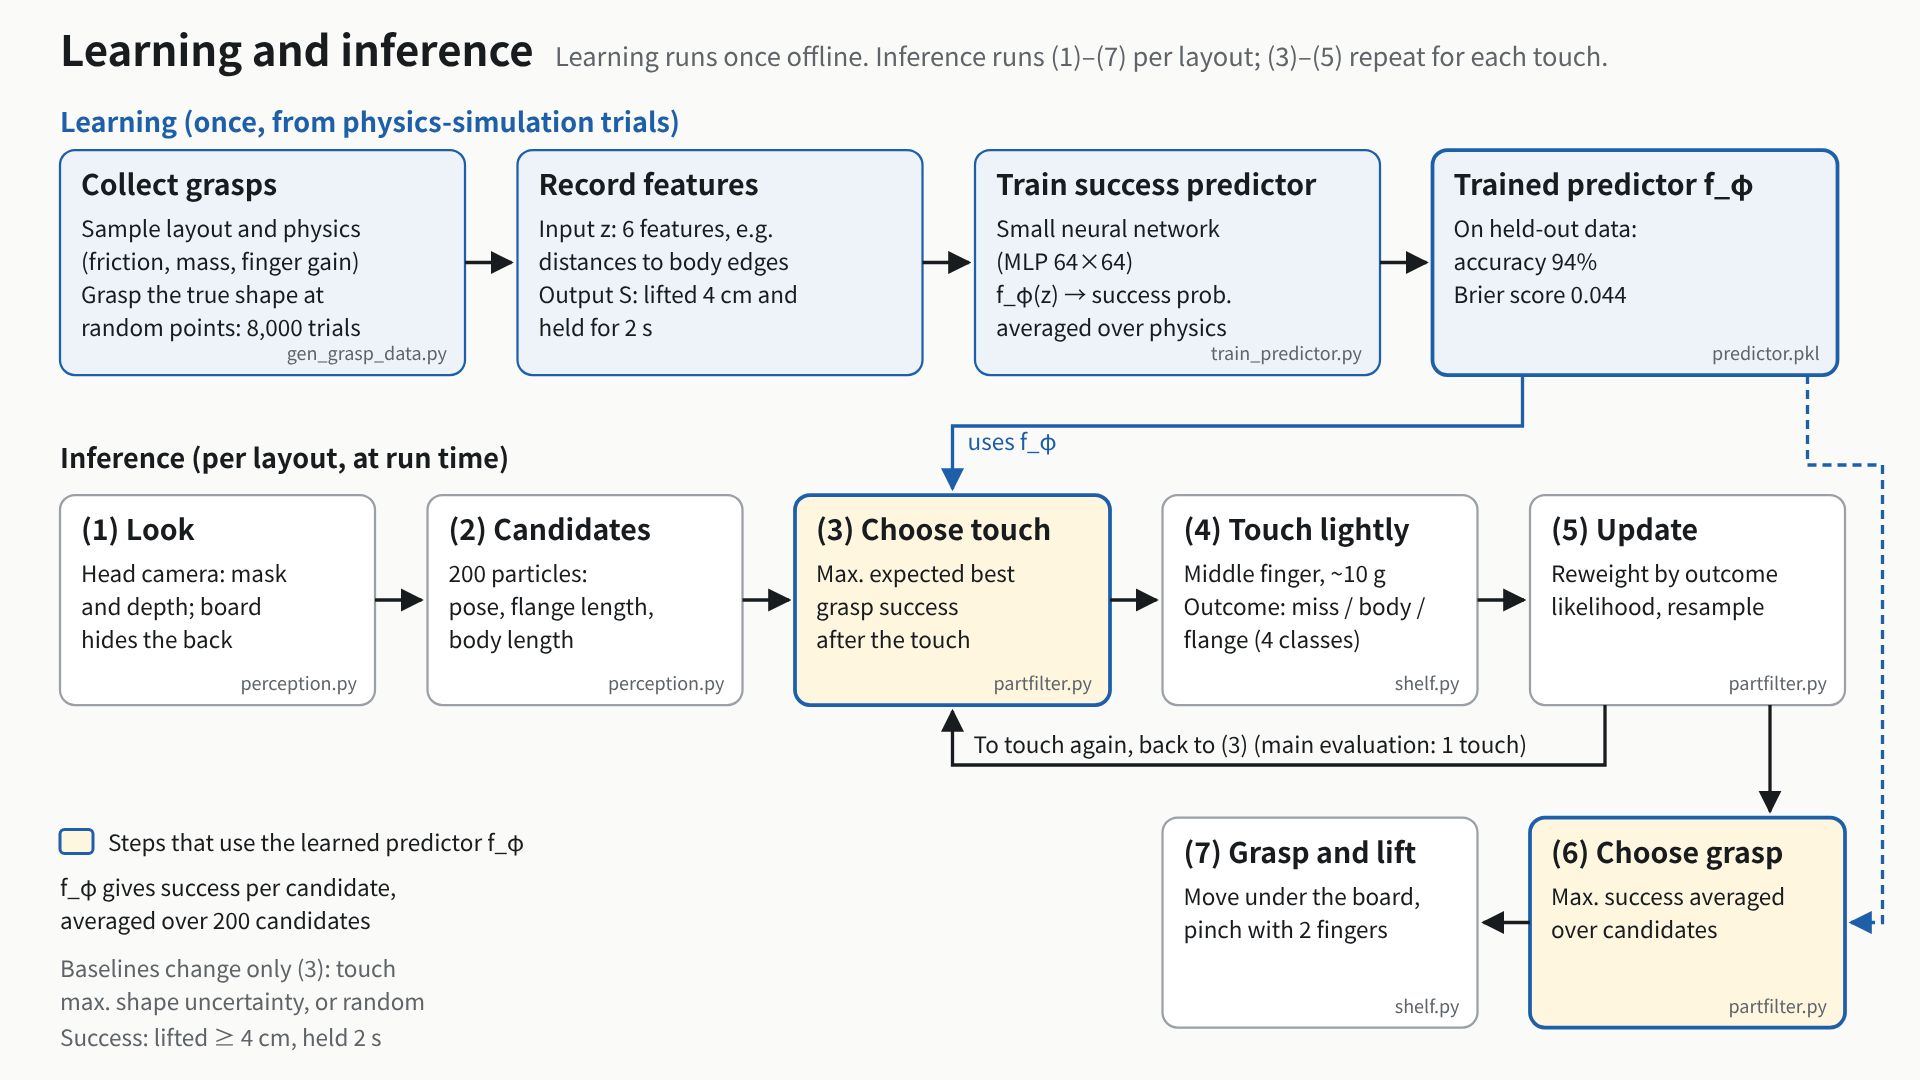
\includegraphics[width=0.92\textwidth]{figures/pipeline.png}
\caption{学習と推論の流れ。上段：成功確率の予測器 $f_\phi$ を、8,000回のシミュレーションの把持から一度だけ学習する（\ref{sec:setup} 節）。下段：配置ごとに、カメラから形の候補を200個作り（\ref{sec:init} 節）、触った後の最良の成功確率の期待値で触る点を選んで触り（\ref{sec:touchsel} 節）、候補を更新し（\ref{sec:obs} 節）、平均した成功確率が最大の点で掴む（\ref{sec:pred} 節）。比較条件の違いは (3) だけである。ファイル名は公開したコードのもの。}
\label{fig:pipeline}
\end{figure*}

\subsection{カメラによる初期化}\label{sec:init}
部品は画像上で幅約20画素と小さく、領域分割の境界の誤りの方が、向きや本体の位置をある程度変えたときのマスクの変化より大きい。そこで深度を次の3つに使う。
(i) \emph{向き}：フランジの高さ（机面から 1.5〜7\,mm）の点を左右 2\,mm の帯に分け、各帯で最も手前の点（5パーセンタイル）を取り、それらを通る直線から手前の縁の向きを得る（開発中の確認で、40配置の平均誤差 2.3$^\circ$、最大 5.1$^\circ$）。
(ii) \emph{位置}：事前分布のまわりから 3,000 個の候補を引き、それぞれについてフランジと本体の箱を投影し、手前の遮蔽物（天板・ロボット）を除いた「見えるはずの領域」を観測のマスクと比べる。境界の1画素は比べない。不一致 $e$ に対する重み $\exp(-(e-e_{\min})/T)$ で 200 個の粒子を選ぶ（同じ確認で、手前の面の平均誤差 1.6\,mm）。
(iii) \emph{本体}：高さ 10\,mm を超える深度の点があれば本体が見えているとみなし、軸に沿って最も手前のその点（30パーセンタイル、真の縁から $\pm$1\,mm 以内）から $\ell_f$ を決める。なければ、高さ 10\,mm の点が天板に隠れ始める線より奥に本体があるとして、$\ell_f$ をその奥側で一様に引き直す。$\ell_b$ は事前分布のままとする。

\subsection{形の候補ごとの把持成功確率の学習}\label{sec:pred}
小さな多層パーセプトロン $f_\phi$ が、候補 $\theta$ を挟む点 $g$ で挟んだときの成功を予測する。入力 $z(\theta,g)$ は6つ：本体の手前の縁から $g$ までの距離、$g$ から本体の奥の縁までの距離、横のずれ、向き、本体の長さ、天板の前端から $g$ までの奥行きである。物理の値 $\xi$ は入力にしないが、学習データの中でばらつかせるので、$f_\phi$ は $\xi$ について平均した成功確率を近似する。信念 $b$ の下で、
\begin{align}
P(S{=}1\mid g,b)&=\frac{1}{N}\sum_{i=1}^{N} f_\phi\bigl(z(\theta_i,g)\bigr),\\
g^*(b)&=\arg\max_{g\in G} P(S{=}1\mid g,b)
\end{align}
とする。$G$ は平均の部品軸に沿って 1\,mm おきに並べた点である。

\subsection{触る観測のモデルと更新}\label{sec:obs}
候補 $\theta$ に対する $u$ の軸方向の座標を $a$、横方向の座標を $c$ とする。結果は、本体の手前の縁までの距離 $a-\ell_f$ と奥の縁までの距離 $a-\ell_f-\ell_b$ で決まる。手前の縁より $-11$\,mm までは指がフランジに当たる。$-11$〜$-3$\,mm では指の腹が本体に当たる。$-3$\,mm から奥の縁の 2\,mm 先までは指先の中央が本体に当たる。奥の縁の 2〜12\,mm 先では再び指の腹が当たる。それより先は外れである。$|c|>W/2+3$\,mm なら何にも当たらない。これらの境界は予備実験で測った値で、それぞれ幅 1\,mm のシグモイドでぼかし、どの結果の確率も0にならないよう、重み $\epsilon=0.02$ で一様分布と混ぜる。触った後は、粒子を $P(o\mid u,\theta_i)$ で重み付けして引き直し、小さな揺らぎを加える。

\subsection{触る点の選択}\label{sec:touchsel}
触る点の候補 $u$ ごとに、各結果の確率と、その結果で更新した後の最良の成功確率を計算し、
\begin{equation}
u^*=\arg\max_{u\in U}\sum_{o} P(o\mid u,b)\,\max_{g\in G} P(S{=}1\mid g,b_{u,o})
\label{eq:voi}
\end{equation}
を選ぶ。$U$ は平均の軸に沿って 3\,mm おきの点、$b_{u,o}$ は $u$ で $o$ を観測した後の信念である。候補×挟む点の成功確率の行列は一度だけ計算し、各 $b_{u,o}$ は行の重みを変えるだけで得られる。

\textbf{比較条件。} \Unc{}（形の不確かさ最大）は、$u$ の真下に本体がある粒子の割合を $p(u)$ として、$p(u)(1-p(u))$ が最大の所を触る。これは Act-VH~\cite{rustler2022actvh} の占有の分散の基準を本問題に当てはめたものである。\Rand{} は $U$ から一様に選ぶ。\Geom{} は、同じ先読み (\ref{eq:voi}) と同じ掴む点の選び方を使うが、$f_\phi$ を境目3つの見積もりに置き換える。$g$ が本体の手前の縁より 3.5\,mm 以上奥、奥の縁より 2.5\,mm 以上手前、横のずれが 5\,mm 以内なら成功とする。境目は本研究の前に、同じシミュレーションでの数十回の予備的な試し掴み（縁の近くで挟む点を 1.5\,mm ずつずらした）から決め、少しの余裕を足したものである。\Fix{} は、ニューラルネットと先読みはそのままで、$\ell_f$ と $\ell_b$ を範囲の中央（20\,mm と 16\,mm）に固定し、カメラ画像との照合でも触った後でも位置と向きだけを推定する。\ref{sec:init} 節の深度による本体の探索は形の推定にあたるので行わない。\Fix{} は、DA-GRD~\cite{wang2026dagrd} のように物体の形を既知として位置を絞り込む方法にあたる。規則 (\ref{eq:voi}) 自体は候補ごとの成功確率の見積もりしか必要とせず、どの比較でも変わらない。

\subsection{触る動作}\label{sec:touchmotion}
触る動作は、部品を動かさないよう約 10\,g で止める。手首は掴むときの向きのまま親指を上げ、中指の先を本体の上面の 1\,cm 上から 1\,mm ずつ下ろし、接触力が 0.1\,N を超えたら止める。部品に当たらず机まで届けば外れとする。結果は、接触が指先の中央から 4\,mm 以内かどうかと、当たった形状（本体かフランジか）で分ける。実機では、感圧センサーの接触位置と接触時の指先の高さを使うことを想定している。触った後は、指先を触り始めの高さに戻し、腕は天板の下のまま、次の触る点か掴む点へ水平に移る。

\section{実験設定}\label{sec:setup}

\begin{table}[t]
\caption{シミュレーションの設定}
\label{tab:setup}
\centering
\small
\begin{tabular}{@{}p{0.2\linewidth}p{0.74\linewidth}@{}}
\toprule
シミュレータ & MuJoCo~\cite{todorov2012mujoco} 3.14、刻み 2\,ms、楕円の摩擦錐、impratio 10、部品にねじり摩擦 \\
ロボット & MuJoCo Menagerie~\cite{menagerie2022} の Unitree G1 と Dex3（3指）。骨盤を固定し、全身に重力補償 \\
把持 & 中指と親指で挟む（人差し指は握り込む）。逆運動学は mink~\cite{zakka2024mink}（右腕7関節） \\
棚 & 机の高さ 0.80\,m、天板はその 20\,cm 上（厚さ 1.5\,cm）。部品の手前の面はロボットの前方 31\,cm・右 25\,cm \\
カメラ & 頭部の D435i 相当、640$\times$480。領域分割の境界に $\pm$1画素の誤り、深度の雑音 $\sigma(z)=z^2\cdot0.08/(f b)$ \\
物理 $\xi$ & 摩擦 0.3〜1.0（指と部品）、部品の質量 $\pm$30\%、指のゲイン $\pm$20\%。配置ごとに引く \\
配置 & $\ell_f,\ell_b$ は一様、向き $\pm20^\circ$、横 $\pm10$\,mm、$v$ は4段階を順に。乱数の種は固定し全規則で共通 \\
予測器 & 真の形をランダムな点で掴んだ 8,000回。MLP 64$\times$64（scikit-learn~\cite{pedregosa2011sklearn}）。確認用データで正解率 94\%、Brier 0.044 \\
\bottomrule
\end{tabular}
\end{table}

設定を表~\ref{tab:setup} に、詳細を付録~\ref{app:setup} に示す。

\textbf{触る点の選び方（主な比較）。} 240配置のそれぞれで、各規則（\Ours、\Unc、\Rand、\Geom、\Fix）が最大2回触り、各回の後の $g^*$ での把持を記録する。認識、予測器、掴む点の選び方は共通である。ただし \Geom{} は、触る点と掴む点の両方を境目の見積もりで選ぶ。

\textbf{触る回数と止め方。} 最初の120配置で、\Ours{} が最大4回触り、各回 $k=0,\dots,4$ の後の把持を記録する。ここから、触らない（A）、$n$ 回触る（B$n$）、予測した成功確率が初めて $\tau$ に届いた時点で止める（C($\tau$)、最大4回）を計算する。触る点の選び方は $\tau$ によらないので、これは各条件を別々に実行するのと同じになる。

\textbf{分岐。} 各把持はシミュレーションの状態の複製の上で行い、触る動作は元の状態から続ける。開発中に、同じ状態から2回掴むと同じ結果になること、複製した場合と複製しない場合が一致することを確かめた。

\textbf{指標。} 主な指標は1回触った後の把持成功率である。差は配置ごとに対応させ、配置についてのブートストラップの 95\% 信頼区間（3,000回、表~\ref{tab:count} では 2,000回）と、片方だけ成功した配置への McNemar の正確検定を用いる。

\section{結果}

\subsection{どこを触るか}

\begin{figure}[t]
\centering
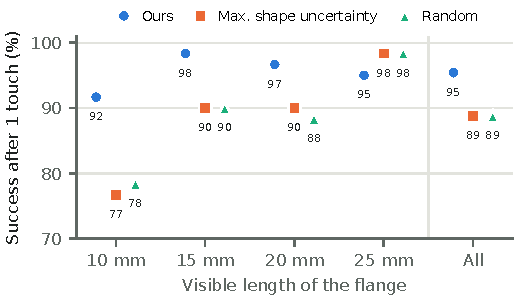
\includegraphics[width=\linewidth]{figures/success_by_vis.pdf}
\caption{見え方ごとの、1回触った後の把持成功率（240配置、各段階60）。\Geom{} は \Ours{} と同じ先読みで、ニューラルネットの代わりに境目3つの見積もりを使う。}
\label{fig:vis}
\end{figure}

1回触った後の成功率は、\Ours{} 95.4\%、\Unc{} 88.8\%、\Rand{} 88.8\% であった（図~\ref{fig:vis}）。\Unc{} に対する対応のある差は +6.7 ポイント（95\% 信頼区間 [+2.1, +11.3]、片方だけ成功した配置 23 対 7、McNemar $p=0.005$）、\Rand{} に対しても +6.7（[+2.5, +11.3]、23 対 7、$p=0.005$）であった。差は見えにくいほど大きく、\Unc{} に対して $v=10$\,mm で +15.0 [+3.3, +26.7]、15\,mm で +8.3 [0.0, +16.7]、20\,mm で +6.7 [0.0, +15.0]、25\,mm で $-3.3$ [$-8.3$, 0.0] であった。25\,mm では本体の手前の縁がカメラに見えることが多い。

1回触った後の、本体の手前の縁の推定の標準偏差（中央値）は、\Ours{} 2.7\,mm、\Unc{} 3.0\,mm、\Rand{} 3.1\,mm であった。形の精度の差は、把持成功率の差に比べて小さい。2回触った後の成功率は 95.0\%、91.7\%、88.3\% で、\Unc{} との差は +3.3 [0.0, +7.1]（$p=0.12$）に縮んだ。\Unc{} も2回目には必要な所に届くためである。

\begin{figure*}[t]
\centering
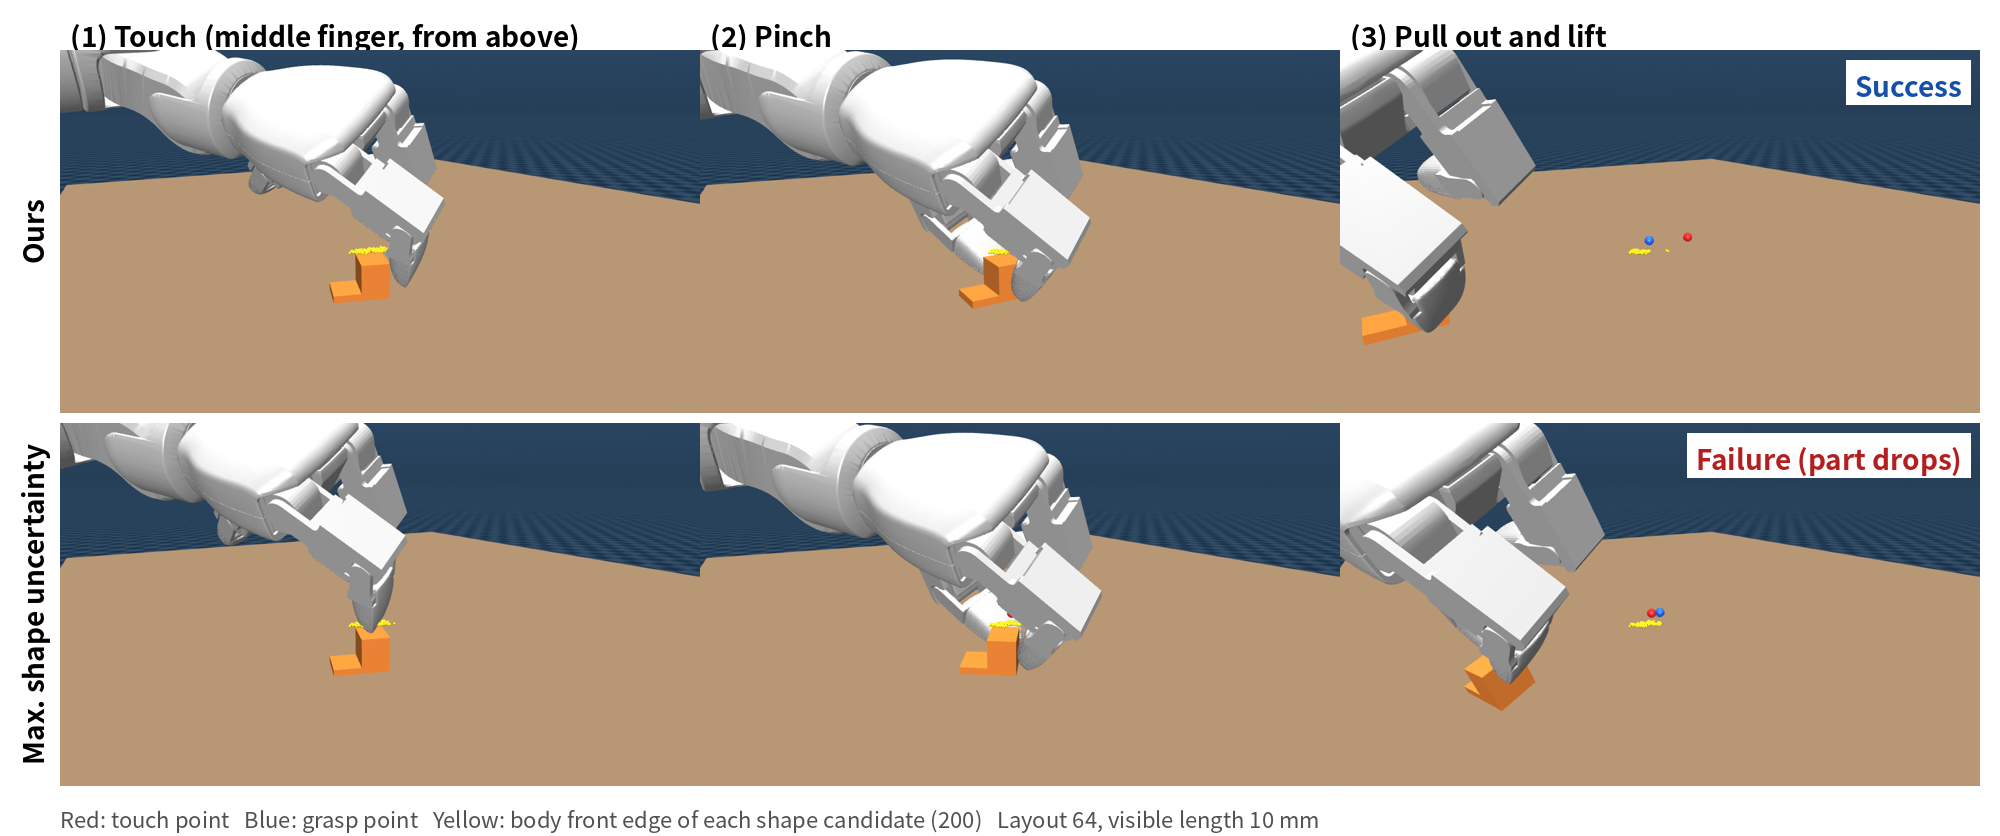
\includegraphics[width=0.95\textwidth]{figures/layout64.png}
\caption{配置64（$v=10$\,mm、本体は手前の面から 15〜31\,mm）。上：\Ours{} は手前の面から 43\,mm、本体の奥の端より先を触って外れる。「本体はそこまで奥にない」と分かって本体の手前の縁のばらつきが 2.9\,mm に縮み、掴める。下：\Unc{} は本体の真ん中（23\,mm）を触って当たるが、手前の縁には 4.3\,mm のばらつきが残り（予測した成功確率 0.63）、掴み損ねる。}
\label{fig:layout64}
\end{figure*}

図~\ref{fig:layout64} は、1つの配置での違いを示す。\Unc{} は本体が「ありそうでなさそうな」所を触るので、本体があることは確かめられるが、挟む点を決める手前の縁についてはあまり分からない。\Ours{} は、結果によって掴む点の選び方が最も変わる所を触る。この配置ではそれが本体の奥の端より先で、外れという結果から、本体とその手前の縁がより手前にあることが分かった。奥側を触るのは一例で、多くの配置では \Ours{} は手前の縁の近くを触る（\ref{sec:disc} 節）。

\begin{table*}[t]
\caption{触る規則：それぞれが何を推定し、どう触る点を選ぶか、および1回・2回触った後の把持成功率（240配置、対応あり）。最後の列は1回触った後の \Ours{} とその規則の差と、95\% ブートストラップ信頼区間。}
\label{tab:rules}
\centering
\small
\begin{tabular}{@{}lllllll@{}}
\toprule
規則 & 隠れた形を推定 & 触る基準 & 成功確率の見積もり & 1回 & 2回 & \Ours{} $-$ 規則 \\
\midrule
\Ours & する & 掴むための先読み & ニューラルネット & 95.4\% & 95.0\% & --- \\
\Geom & する & 掴むための先読み & 境目3つ & 93.8\% & 94.2\% & +1.7 [$-$1.3, +4.6] \\
\Fix & しない（中央の寸法） & 掴むための先読み & ニューラルネット & 76.7\% & 79.6\% & +18.8 [+12.9, +25.0] \\
\Unc & する & 形の不確かさ & ニューラルネット & 88.8\% & 91.7\% & +6.7 [+2.1, +11.3] \\
\Rand & する & ランダム & ニューラルネット & 88.8\% & 88.3\% & +6.7 [+2.5, +11.3] \\
\bottomrule
\end{tabular}
\end{table*}

\subsection{隠れた形の推定}\label{sec:fix}
表~\ref{tab:rules} にすべての規則をまとめる。形を中央の寸法に固定すると（\Fix）、1回触った後の成功率は 76.7\% で、\Ours{} より 18.8 ポイント低く（95\% 信頼区間 [+12.9, +25.0]、片方だけ成功 53 対 8、McNemar $p<0.001$）、\Unc{} と比べても 12.1 ポイント低かった（[$-$17.9, $-$6.2]、$p<0.001$）。差は $v=10$\,mm で最も大きかった（+26.7 [+13.3, +40.0]）。これは予想どおりである。形を固定すると、本体の縁が想定と違う所で見つかったとき、部品全体の位置がずれたとしか説明できず、カメラで見えているフランジの位置と食い違う。この比較は、掴める所が隠れている部品では、掴むための触る規則は位置だけでなく隠れた形も推定しなければならないことを確かめるものである。

\subsection{簡単な見積もりと細かい見積もり}\label{sec:geom}
$f_\phi$ の代わりに境目3つの見積もりを使うと（\Geom）、1回触った後の成功率は 93.8\% で、\Ours{} の 95.4\% との差は +1.7 ポイント（95\% 信頼区間 [$-$1.3, +4.6]、片方だけ成功 9 対 5、McNemar $p=0.424$）であった。見え方ごとの \Ours{} と \Geom{} の差は、10\,mm で +1.7 [$-$3.3, +6.7]、15\,mm で +0.0 [$-$5.0, +5.0]、20\,mm で +3.3 [$-$3.3, +10.0]、25\,mm で +1.7 [$-$5.0, +8.3] であった。2回触った後は 95.0\% 対 94.2\%（+0.8 [$-$2.5, +4.6]、$p=0.815$）であった。\Geom{} も \Unc{} より 5.0 ポイント高かった（[+0.4, +10.0]、22 対 10、$p=0.050$）。1回触った後の本体の手前の縁のばらつきの中央値はどちらも 2.7\,mm で、実行した把持の予測確率の Brier スコアは \Ours{} 0.046、\Geom{} 0.061 であった。どちらの見積もりでも、\Unc{} や \Rand{} との差を生んでいるのは掴むための先読みである。信頼区間からは、ニューラルネットに数ポイントの利点がある可能性は否定できない。

\subsection{何回触るか、いつやめるか}

\begin{table}[t]
\caption{触る回数と止め方（120配置）}
\label{tab:count}
\centering
\small
\begin{tabular}{@{}lccc@{}}
\toprule
条件 & 成功率 & 触った回数 & $v$ = 10/15/20/25\,mm \\
\midrule
A：触らない & 72.5\% & 0 & 53 / 63 / 77 / 97\% \\
B1：1回 & 96.7\% & 1 & 90 / 100 / 97 / 100\% \\
B2：2回 & 94.2\% & 2 & 87 / 97 / 97 / 97\% \\
B3：3回 & 96.7\% & 3 & 97 / 97 / 100 / 93\% \\
C(0.85) & 95.0\% & 0.96 & 90 / 100 / 97 / 93\% \\
C(0.95) & 94.2\% & 1.61 & 93 / 100 / 97 / 87\% \\
\bottomrule
\end{tabular}
\end{table}

触らないと成功率は 72.5\% で、$v=10$\,mm では 53\% まで下がった（表~\ref{tab:count}）。1回触ると 96.7\% に上がり、それ以上触っても上がらなかった。閾値の規則 C は、$v=25$\,mm ではしばしば触らずに掴んだが、その分わずかに失敗が増え、全体では B1 を上回らなかった（C(0.85) と B1 の差 $-1.7$ ポイント [$-4.2$, 0.0]、触った回数の差 $-0.04$ 回）。

\subsection{較正}

\begin{figure}[t]
\centering
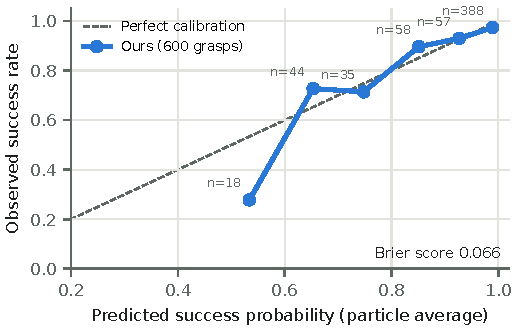
\includegraphics[width=0.95\linewidth]{figures/calibration.pdf}
\caption{粒子で平均した成功確率の較正（120配置 $\times$ 5時点 = 600回の把持）。}
\label{fig:calib}
\end{figure}

粒子で平均した成功確率は、実際の成功率とよく一致した（図~\ref{fig:calib}、Brier 0.066）。予測 0.9 以上が把持の 74\% を占め、その実際の成功率は 93〜97\% であった。0.6 未満の区間（18回）だけが楽観的であった（実際 28\%）。学習データと同じ分布の確認用データでは Brier 0.044 なので、全体の流れの中の推定の誤差で較正が崩れることはなかった。学習データの把持は触らずに天板の手前から差し込んだものだが、触った後に天板の下から始まる把持でも較正は保たれた。

\subsection{失敗の損と時間}\label{sec:cost}
失敗した把持では、部品が大きく動いた。120配置では失敗55回の 91\% で部品が 10\,mm 以上動き（中央値 約 250\,mm）、240配置の比較では（\Ours、\Unc、\Rand{} と両方の回をまとめて）失敗125回の 98\% で 10\,mm 以上動いた（中央値 約 140\,mm）。手を引き出すときに部品を引きずるか弾くためである。触る押し下げの間の部品の移動は最大 0.33\,mm、指の接近と引き上げを含めても最大 2.3\,mm であった。触った後は腕を天板の外へ戻さず天板の下に置いたままにし、この動きで開始から掴み終わる（2秒保持の終わり）までの時間の中央値は、1回触る場合 15.2 秒、2回触る場合 17.7 秒であった（20配置、\Ours）。

\section{考察と限界}\label{sec:disc}

\textbf{なぜ1回で足りるのか。} ここで成否を決めるのは主に本体の手前の縁の位置で、挟む点はそこから 3.5\,mm 以上奥、奥の縁から 2.5\,mm 以上手前になければならない。\Ours{} は、結果によって候補が分かれる所、つまり本体の縁のまわりを触る。1回目の触りのうち 59\% は本体の外（手前の縁より 3\,mm 以上手前、または奥の縁より 5\,mm 以上奥）で、本体の中央から 5\,mm 以内は 4\% だけであった。結果は、指の腹で本体 46\%、指先の中央で本体 38\%、フランジ 10\%、外れ 6\% に分かれた。指の腹やフランジに当たったという結果が、指が縁のどちら側にあったかを教える。\Unc{} が本体の外を触ったのは 18\% だけで、73\% で指先の中央が本体に当たった。本体があることは確かめられるが、手前の縁の位置はあまり絞れない。この違いは形の精度（2.7 対 3.0\,mm）より把持成功率にはるかに大きく表れ、探索の目的を形の復元ではなく後の把持に置くことを支持する。

1回で足りるのは、部品の奥行きの形（手前にフランジ、奥に本体）が既知で、未知の範囲が短いためである。カメラで位置と向きが決まると、残る未知は主に約 20\,mm の範囲にある本体の手前の縁で、本体の内側の掴める幅は 6\,mm 以上ある。縁のどちら側に当たったかが分かる1回の触りで、掴む点を内側に置ける。型の分からない部品や、未知の範囲が長い部品では、もっと触る必要があるかもしれない。

\textbf{成功確率の見積もりはどこまで細かくあるべきか。} 2つの見積もりはどちらも同じシミュレーションの把持から作ったもので、違いは大きさ（数十回の試行から決めた境目3つと、8,000回から学習したニューラルネット）と出力（候補ごとに0か1か、確率か）である。この部品では、隠れた形が分かれば、掴めるかどうかは挟む点が本体の縁からどれだけ内側にあるかでほぼ決まり、それは境目3つで表せる。この部品はニューラルネットを要するほど難しくなく、ニューラルネットとの差は +1.7 ポイント（有意差なし）で、Brier スコアはやや低かった。より細かい見積もりが意味を持つのは、掴める範囲が縁からの距離以外でも決まる部品である。たとえば重心が偏っていると、最良の挟む点が隠れた長さの比で変わる。その利点は全体が見えている部品でも生じ、学習した把持の質のモデル~\cite{mahler2017dexnet2} と同じである。本研究の規則が加えるのは、見積もりが重要だとする所を、規則を変えずに触りが狙う、という点である。

\textbf{なぜ止める判断が効果を持たなかったか。} うまく選んだ1回の触りで成功率はほぼ上限（約 97\%）に届き、残った少数の失敗（B1 で120回中4回）は、記録した物理の値に共通の原因が見当たらない。結果が当たり／外れだけの場合や未知の量が多い場合には、止める判断で成功率を保ったまま触る回数を減らせる可能性があるが、本研究では確かめていない。

\textbf{触ると部品が動く。} 推定は部品が動かないと仮定している。初期の実装では、触るたびに引き上げる途中で指が部品を約 1\,mm 引きずるのが観察され、触るほど誤差が積み重なった。指を細かい刻みで真上に引き上げ、天板の下では指を下げないようにした後は、部品の移動は押し下げの間で最大 0.33\,mm、接近と引き上げを含む触り全体で最大 2.3\,mm になった。部品の動きを推定に含めることは今後の課題である。

\textbf{結論は腕の動きによらない。} 触るたびに腕を天板の下から外へ戻していた初期の動きで同じ実験を行うと、1回触った後の成功率は \Ours{} 95.8\%、\Unc{} 90.0\%、\Rand{} 88.3\%（\Unc{} に対して +5.8 [+1.7, +9.6]、$p=0.007$）、触らない場合 72.5\%、1回触る場合 95.8\% であった（付録~\ref{app:v1}）。

\textbf{限界。} 第一に、結果はすべてシミュレーションである。観測の境界と把持の許容幅はシミュレーションの指の形と接触モデルに依存し、実機の感圧センサーや摩擦は、ばらつかせた範囲の外にある可能性がある。第二に、形の型は既知で、未知は2つの長さだけである。ほかの型の部品には、CAD から作る形の族や、ニューラルネットによる形の補完~\cite{rustler2022actvh,rustler2026shapegrasp} の候補が必要になる。触る点の選び方は、候補の表し方によらない。第三に、\Unc{} は Act-VH の基準を本問題に当てはめて再実装したもので、元の手法そのものではない。第四に、触る点の候補は1次元の軸上に限られる。第五に、手の経路と指の開閉は決めうちである（決めた経由点を逆運動学で解く）。学習と推論で決めるのは触る点と掴む点だけなので、規則の違いは触る場所だけで、成功率の差はその選び方だけから生じる。一方で、天板や隣の物を避ける経路の計画はしておらず、実機では関節の追従の遅れや指先の摩擦の低さのために、同じ決めうちの動作でも失敗しやすくなる可能性がある。動きを遅くすればこれは減るが、上で述べた時間の短縮は小さくなる。

\section{まとめ}

棚の天板で奥が隠れた部品を掴むために、形の候補で平均した、触った後の最良の把持成功確率の期待値で触る場所を選んだ。240の対応のある配置で、こうして選んだ1回の触りの後の把持成功率は 95.4\% で、形の不確かさが最大の所を触る場合の 88.8\%、ランダムの 88.8\% を上回り、見える部分が少ないほど差が大きかった。ニューラルネットの代わりに境目3つの見積もりを使うと 93.8\% で、この部品の族は細かい見積もりを必要とせず、成功率の差は触る場所から生じていた。形を中央の寸法に固定して位置だけを推定すると 76.7\% で、隠れた形を信念に含める必要がある。形を補うために触るときは、形が最もよく復元できる所ではなく、結果によって掴む点の選び方が最も変わる所を触るべきである。実機での検証、より広い形の族、触る動作による部品の動きの推定への取り込みが今後の課題である。

\section*{謝辞}
著者は、コードの実装、シミュレーション実験の実行、図の作成、本文の下書きと翻訳に Claude（Anthropic）を用いた。課題の設定、手法と比較の選択、結果の解釈、すべての内容の確認と修正は著者が行い、その内容に全責任を負う。

\bibliographystyle{IEEEtran}
\bibliography{refs}

\appendix

\section{設定の詳細}\label{app:setup}

\textbf{シーン。} Dex3 ハンド付きの G1 のモデルは MuJoCo Menagerie~\cite{menagerie2022} のコミット \texttt{c96a32d} のものを使う。骨盤は世界に固定し、重力補償は全身に掛ける（右腕だけに掛けると腰が約 4$^\circ$ たわみ、頭部カメラが傾いた）。左腕は机に触れない位置に動かす。頭部カメラは Unitree の URDF の D435i の取り付けに従う（約 48$^\circ$ 下向き、縦の視野角 58$^\circ$）。部品は2つの箱からなる1つの剛体で（密度 600\,kg/m$^3$、\texttt{condim}=4 でねじり摩擦あり）、フランジの箱は本体と 1\,mm 重なる。

\textbf{見え方。} 見える長さ $v$ に対し、頭部カメラから天板の前端の下の角を通る光線が、部品の手前の面から $v$ 奥でフランジの上面に届くように天板の前端を置く。

\textbf{把持の動作。} 手首は $-60^\circ$ のロール、$10^\circ$ のピッチ、鉛直軸まわり $-55^\circ$ のヨーとし、挟む軸がほぼ左右方向になるようにする。人差し指は握り込む。触る前の把持では、天板の 10\,cm 手前から、挟む点の 20\,mm 上の高さで水平に手を差し込み、下ろす。触った後は、天板の下で今の高さ以上を保って挟む点の上へ移る。親指と中指はそれぞれ独立に閉じ、接触したら止める。両方が触れたら、0.3 秒かけて決まった量だけさらに締める。その後、部品を 1\,cm 浮かせ、天板の 10\,cm 手前まで引き出し、挟む高さの 6\,cm 上まで持ち上げて2秒保持する。天板の近くと下での移動は、デカルト空間の直線を経由点に分け（既定 15、触る下降では 1\,mm ごとに1点、引き上げでは 12）、それぞれを mink~\cite{zakka2024mink} で解き、関節の目標を時間に沿って線形補間する。空いた空間での移動（天板の手前での接近と手首の向きの変更）は、逆運動学を一度解いて関節空間で補間する。

\textbf{物理のばらつき。} 配置ごとに、摩擦係数 $\mu\sim U[0.3,1.0]$ を指と部品に入れる（MuJoCo は接触する2つの形状の大きい方を使う）。部品の質量と慣性は $U[0.7,1.3]$ 倍、手のアクチュエータの位置ゲインは $U[0.8,1.2]$ 倍にする。質量を変えた後は MuJoCo の派生定数を計算し直す。そうしないとシミュレーションが不安定になり、成功率が見かけ上下がる。

\textbf{カメラのモデル。} 領域分割はシミュレータの正解をもとに、マスクを1画素縮めるか広げ（それぞれ確率 1/3、残りはそのまま）、境界の画素の 30\% を反転して崩す。深度の雑音は D435i のモデル $\sigma(z)=z^2\cdot0.08/(f b)$（基線長 $b=50$\,mm）に従う。

\textbf{パーティクルフィルタ。} 事前の候補 3,000 個：手前の面の位置は奥行き方向に $\mathcal{N}(\text{事前},\,(30\,\text{mm})^2)$、左右に $\mathcal{N}(\text{事前},\,(15\,\text{mm})^2)$、向きは深度による推定のまわりに $\mathcal{N}(\hat\psi,\,(3.5^\circ)^2)$、$\ell_f\sim U[10,30]$\,mm、$\ell_b\sim U[12,20]$\,mm。照合の温度 $T=0.05$。揺らぎ（0.5\,mm、1$^\circ$）を加えて 200 個の粒子を引く。触るたびに揺らぎ（0.3\,mm、0.5$^\circ$）を加えて引き直す。掴む点の候補は 1\,mm おき、触る点の候補は 3\,mm おきで、平均の手前の面から 0〜55\,mm の範囲に置く。

\textbf{予測器の学習。} 8,000回の学習用の把持は、それぞれ上と同じように配置を引き、真の形を、軸方向の位置 $a\sim U[\ell_f-6\,\text{mm},\ \ell_f+\ell_b+4\,\text{mm}]$、横のずれ $U[-8,8]$\,mm、高さの誤差 $\mathcal{N}(0,(1\,\text{mm})^2)$ で挟む。全体の成功率は 48\% であった。MLP は 64 ユニットの隠れ層2つ（$\alpha=10^{-3}$、早期終了）で、特徴は mm と度にそろえて標準化する。前の 80\% で学習し、後ろの 20\%（1,600回）で確かめると、正解率 0.943、Brier 0.044 であった。公開したモデルは 8,000回すべてで学習し直したものである。

\textbf{触る観測の境界。} $d_f=a-\ell_f$、$d_b=a-\ell_f-\ell_b$ とすると、$a\ge0$ かつ $d_f<-11$\,mm で \textsc{flange}、$-11\le d_f<-3$\,mm で \textsc{body-other}、$d_f\ge-3$\,mm かつ $d_b<2$\,mm で \textsc{body-center}、$2\le d_b<12$\,mm で \textsc{body-other}、それ以外か横のずれが $W/2+3$\,mm を超えると \textsc{miss} である。シミュレータでは、\textsc{body-center} は指先の中央から 4\,mm 以内の本体への接触で、触る動作は 0.1\,N で止まる。

\section{初期の腕の動きでの結果}\label{app:v1}
初期の実装では、触るたびに腕を天板の下から外へ戻して差し込み直し、親指もすぐに掴む形に戻していた。その動きでは、1回触った後の成功率は \Ours{} 95.8\%、\Unc{} 90.0\%、\Rand{} 88.3\% で、\Unc{} に対する対応のある差は +5.8 ポイント [+1.7, +9.6]（$p=0.007$）であった。触る回数の実験では、触らない場合 72.5\%、1回触る場合 95.8\% であった。どちらの生の結果もリポジトリにある（\texttt{results/v1\_retract/}）。別に行った20配置の時間の計測（保存していない）では、初期の動きの所要時間の中央値は1回触る場合 17.7 秒、2回触る場合 24.3 秒で、本論文の動きでは 15.2 秒と 17.7 秒であった。

\section{視覚言語モデルとの組み合わせ}\label{app:vlm}
本手法が決めるのはどこを触りどこを挟むかで、どの部品を取るかは決めない。そこで、指示文から部品を選ぶ SmolVLM~\cite{marafioti2025smolvlm} と組み合わせた。色と隠れたサイズの違う2つの部品を、天板の下に 10\,cm 離して置く（5\,cm では手が隣の部品に当たった）。天板の前端は共通なので、どちらもフランジの同じ長さがカメラに見え、サイズの違いは見えない。SmolVLM-500M に、部品の上に番号を描いて切り出し拡大した頭部カメラの画像と、英語の指示文（例："Pick up the green part."）を与え、番号で答えさせる。選ばれた部品を本手法で触ってから掴む。著者の GPU での3回の実行（指示文の色を変えた場合と位置を入れ替えた場合を含む）で、SmolVLM-500M は正しい部品を選び、ロボットはそれを持ち上げた。

\begin{figure*}[t]
\centering
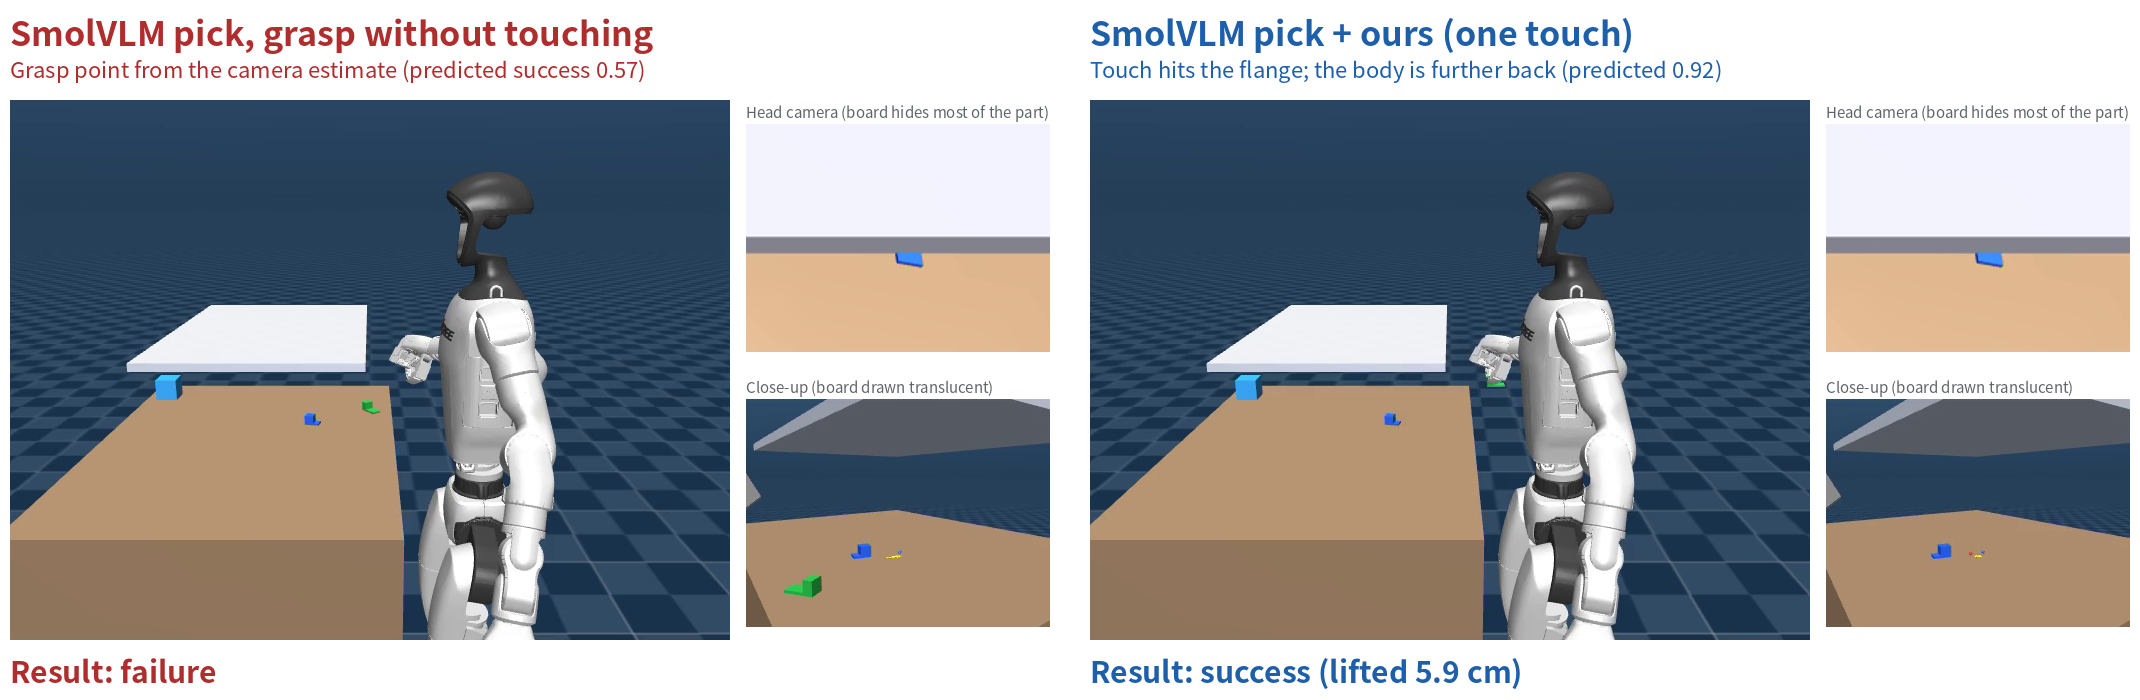
\includegraphics[width=0.95\textwidth]{figures/vlm_compare.png}
\caption{同じ場面、同じ SmolVLM の答え（「2」、緑の部品：フランジ 28\,mm、本体 13\,mm）。左：触らずにカメラの推定から掴むと失敗する。右：1回の触りがフランジに当たり、本体がより奥にあると分かって掴める。腕の動きは同じで、違うのは触るかどうかだけである。}
\label{fig:vlm}
\end{figure*}

次に、選んだ部品の掴み方を 60配置 $\times$ 部品2つ = 120回で比べた（隠れたサイズは予測器の学習範囲から引き、ほかの設定は \ref{sec:setup} 節と同じ）。すべての条件を分岐により同じ観測から評価し、部品の選択は正しいとした。VLM が掴む点を選ぶ条件では、推定した手前の面から 8〜48\,mm の候補点 A〜F（8\,mm おき）を画像に描き、SmolVLM に学習なしで1つ選ばせた。

\begin{table}[h]
\caption{選んだ部品の掴む点の決め方（120回）}
\label{tab:vlm}
\centering
\small
\begin{tabular}{@{}lc@{}}
\toprule
掴む点を決めるもの & 成功率 \\
\midrule
SmolVLM-500M、部品の知識なし & 0.8\% \\
SmolVLM-2.2B、部品の知識なし & 0.8\% \\
SmolVLM-500M、長さの範囲を文で与える & 43.3\% \\
SmolVLM-2.2B、長さの範囲を文で与える & 61.7\% \\
学習した予測器、触らない & 75.8\% \\
本手法、1回触る & 95.0\% \\
\bottomrule
\end{tabular}
\end{table}

部品の知識がないと、SmolVLM-500M は A か F だけ、SmolVLM-2.2B は F だけを答え、ほとんど持ち上がらなかった。フランジと本体の長さの範囲、候補点の距離、必要な余裕を文で与えると中ほどの点を選ぶようになったが、SmolVLM-2.2B の答えは C か D だけで、いつも C（57\%）や D（65\%）を選ぶのと同程度であった。本体は天板に隠れているので、画像には配置ごとに掴む点を変える手がかりがない。同じカメラの推定を使う学習した予測器は 75.8\% で、SmolVLM-2.2B より 14.2 ポイント高かった（片方だけ成功 32 対 15、McNemar $p=0.019$）。1回触ると成功率は 95.0\% になり、触らない予測器より 19.2 ポイント高かった（95\% 信頼区間 [+11.7, +26.7]、片方だけ成功 25 対 2、$p<0.001$）。$v=10$\,mm では 63\% から 93\% に上がった。2つの問いの文は \texttt{run\_vlm\_point.py} にそのまま載せている。

\section{再現}\label{app:repro}
コード、学習済みの予測器、すべての生の結果、動画は \url{https://github.com/Nishina-N/Physics-Informed-Touch-Selection} にある。環境は Python 3.11、MuJoCo 3.14、mink 1.3、scikit-learn 1.8.0（\texttt{uv.lock} で固定）である。
\begin{footnotesize}
\begin{verbatim}
uv sync
git clone https://github.com/google-deepmind/\
mujoco_menagerie third_party/mujoco_menagerie
git -C third_party/mujoco_menagerie checkout \
  c96a32d28fb5da84da38c1da4d749e7a13212855
# 保存済みの結果から数値を出す（数秒）
uv run python analyze_touchsel.py
uv run python analyze_branch.py
# 予測器を学習し直す（数秒）
uv run python train_predictor.py
# すべてやり直す（k = 0..n-1 を並列に）
uv run python gen_grasp_data.py 0 2 8000
uv run python run_touchsel.py 0 2 240 predictor.pkl
TSEL_RULES=geom uv run python run_touchsel.py \
  0 2 240 predictor.pkl
TSEL_RULES=fixshape uv run python run_touchsel.py \
  0 2 240 predictor.pkl
uv run python run_branch.py 0 2 120 predictor.pkl
\end{verbatim}
\end{footnotesize}
期待される出力：\texttt{analyze\_touchsel.py} は成功率 0.954（\Ours）、0.887（\Unc。213/240 = 88.75\% を 88.8\% と表記）、対応のある差 +0.067、McNemar $p=0.005$ を出す。\texttt{analyze\_branch.py} は A 0.725、B1 0.967、C(0.85) と B1 の差を出す。\texttt{paper/make\_numbers.py} と \texttt{paper/make\_figures.py} は比較の数値と結果の図を作り直す。\texttt{train\_predictor.py} は Brier 0.044、正解率 0.943 を出し、\texttt{predictor.pkl} を再現する。配置は乱数の種で固定されているので、配置0をやり直すと保存済みの結果と完全に一致する。1つの CPU コアで、学習データの生成は約 3.5 時間、120配置の触る回数の実験は約 20 分かかる。\texttt{view\_trial.py 64 --rule voi} は図~\ref{fig:layout64} の試行を表示し、\texttt{docs/code\_guide.html} は実行順にコードを解説する。

\end{document}
